\documentclass[12pt]{article}
\usepackage{amsmath}
\usepackage{csvsimple}
\usepackage{graphicx}
\graphicspath{ {./../images/} }
\usepackage{hyperref}
\usepackage[latin1]{inputenc}
\usepackage{listings}

\DeclareMathOperator{\Tr}{Tr}

\lstset{
  columns=fullflexible,
  breaklines=true,
  }

\twocolumn

\title{Local Assortativity in Networks with Unbalanced Classes}
\author{Rebecca Cohen}

\begin{document}
\maketitle
\section{Introduction}

In many network datasets, edges may be more, or less, frequent between pairs of nodes that share a common attribute.  To measure this tendancy on a network with a discrete attributes, we use the normalized modularity score
 \begin{equation}
   r = \frac{Q}{Q_{max}} = \frac{\sum_g e_{gg} - \sum_g a_g^2} {1 - \sum_g a_g^2}
 \end{equation} \cite{newman:2003}
 
 where $e_{gg}$ is the fraction of edges that connect nodes of class $g$, and $a_g$ is the fraction of edges attached on either side to nodes of class $g$.  This statistic provides a global summary of the relation between edges and attribute values across the network.  
 
However, this metric will not capture the variation that occurs within the network.  To capture a more nuanced representation of the assortative behavior in the neighborhood of a fixed node $i$, Peel et al. have proposed a local assortativity measure

\begin{equation}
  r_\ell = \frac{1}{Q_{max}} \sum_g (e_{gg}(\ell) - a_g^2)
\end{equation}

where $e_{gg}(\ell)$ is the fraction of edges connecting nodes in class $g$, weighted by the importance of each endpoint in the neighborhood of $\ell$.  

Personalized PageRank is a popular measure of local node importance in which $w_\alpha(i; \ell)$ is the stationary probability that a random walker beginning at $\ell$ will be at $i$, assuming they teleport back to $\ell$ with probability $1-\alpha$.  When $\alpha$ is close to 0, the bulk of weight is in the immediate neighborhood of $\ell$, while values closer to 1 produce something closer to the global assortativity.  To summarize the behavior across multiple scales, we use the TotalRank

\begin{equation}
  w_{multi}(i; \ell) = \int_0^1 w_\alpha(i; \ell) d\alpha
\end{equation} \cite{boldi:2005} \cite{Peel:2018}

and define
\begin{equation}
  e_{gg}(\ell) = \sum_{i: z_i \in g} \sum_{j: z_j \in g} w_{multi}(i; \ell) \frac{\mathbf{A}_{ij}}{k_i}
\end{equation} \cite{Peel:2018}

where $\mathbf{A}$ is the adjacency matrix, $\vec{k}$ is the degree vector, and $\vec{z}$ is the attribute vector.

Peel et. al find considerable variation in $r_\ell$ on both random and empirical networks.  However, it is not obvious whether local differences in assortativity are the result of differences in the probability of nodes forming in-group vs. out-group edges, or whether there may be other factors that influence the distribution of $r(\ell)$.

This paper will analyze the distribution of $r(\ell)$ with respect to class size.  We find that otherwise comparable nodes in larger classes tend to have higher $r(\ell)$ scores on both assortative and disassortative networks.  We develop a theoretical prediction of $r(\ell)$ based on a DC-SBM null model and use numerical experiments to validate its predictions.

\section{Methods}
To test the influence of class size on local assortativity, we use random graphs in which there is no fine-grained assortative structure and record how $r_\ell$ varies relative to class size.  This experimental setup considers two different null models, the Erdos-Renyi random graph, which has no assortatitive structure, and a simple stochastic block model (SBM) with equal in- and out-group pairing probabilities for all classes of nodes.

The Erdos-Renyi random graphs in this experiment had $N=800$, $p=0.075$, while the SBM had 2 blocks of varying sizes, with $N=800$, with an in-group pairing probability of 0.1 and out-group pairing probability of 0.05.  On both models, nodes were assigned to one of two classes, with the size of the smaller class varying between 10 and 400 by units of 10.  For each choice class size, 20 trials were run on different random graphs and the mean $r_\ell$ was recorded for each class, as was the global assortativity.

We then derive an estimate of the expectation of $r_\ell$ on a network with global assortative structure but no fine-grained variation within each class.  To test the estimates, we fix the proportional sizes of 10 classes as well as in-group and out-group pairing probabilities.  For varying sizes of network, we generate 50 DC-SBM random networks and compare the mean $r_\ell$ values within each class with the estimate.  We also examine the distribution of $r_\ell$ within each class.  

\section{Results}
\subsection{Distribution of $r_\ell$ on Random Graph Models}

\begin{figure}
  \includegraphics[width=0.5\textwidth]{erdos_renyi_{date_str}.png}
  \includegraphics[width=0.5\textwidth]{unbalanced_sbm_2021_11_30_13_01.png}
  \caption{Distribution of $r(\ell)$ on Erdos-Renyi random graphs (top) and SBM's (bottom).  Error bars indicate the standard deviation of the mean $r(\ell)$ for each class between trials.}
\end{figure}


Figure 1 shows the results of the experiment.  On both null models, the larger class consistently had higher $r(\ell)$ scores than the smaller one.  The steep dropoff in $r(\ell)$ as the smaller class size decreases is striking in both experiments.  Neither network had disassortative structure, yet as the size of the smaller group approaches 0, $r(\ell)$ approaches $-\infty$.  The precipitous drop in score has to do with the normalization term.  Without loss of generality, suppose the largest group is group 1.  As the size of group 1 approaches the entire dataset, $a_1 \to 1$, so
\begin{equation}
  Q_\text{max} = 1 - \sum_g a_g^2 \to 1 - 1 = 0 
\end{equation}

The normalization term explains the magnitude of the decline in $r_\ell$, but to understand why it is negative to begin with we must consider what happens to $e_{gg}(\ell)$ as class sizes become increasingly unbalanced.  Consider a node $\ell$ in group 1, the larger group.  TotalRank will assign a higher weight to node $\ell$ than to any other node, thus edges connecting node $\ell$ to other nodes in group 1 will be given the most weight in $e_{11}(\ell)$, leading to a higher proportion of in-group edges than expected even when there is no assortative structure.  Internal edges in group 2 will be given weight less than $a_2^2$ but these are a smaller fraction of the network so this different will be outweighted by the results from group 1.

Conversely, if we take $\ell$ in group 2, the smaller group, then $e_{22}(\ell)$ will be greater than $a_2^2$, but this will be outweighed by the large defecit in $e_{11}$ as none of the top-weighted edges can be internal to group 1.

Also worth noting here is that global assortativity scores depend on class size as well, reaching a maximum when classes have equal sizes.  While it is tempting to search for class-size correction that could be applied $r(\ell)$, the assumption that variation on modularity could be independent of class size may be misguided.  

\subsection{Baseline $r(\ell)$ Scores}

In order to draw conclusions about local differences in node pairing behaviors, we would like to be able to distinguish between variance in $r(\ell)$ due to class size vs. fine-grained differences in behavior.  

The multiscale mixing score $r(\ell)$ is defined
\begin{equation}
  r(\ell) = \frac{1}{Q_{max}} \sum_g (e_{gg}(\ell) - a_g^2)
\end{equation}

where 
\begin{equation}
  e_{gg}(\ell) = \sum_i \sum_j w_{\text{multi}}(i; \ell) \frac{A_{ij}}{k_i} \delta(z_i, z_j) 
\end{equation}

and $k_i$ is the degree of the ith node, while $w_{\text{multi}}(i; \ell)$ is the $i$th element of the totalRank vector centered at node $\ell$.  With two key assumptions, we can calculate the expectation of $r(\ell)$ under a degree-corrected stochastic block model (DC-SBM).  While neither is assumption is true in general, numerical simulations support the predictions resulting from this calculation:

\begin{enumerate}
  \item The degree of every node is equal to its expected degree ($k_i = \theta_i$)
  \item The network is fully connected
\end{enumerate}

Assumption 1 allows us to treat node degrees and edge counts as constants.  Without this assumption, both $e_gg(\ell)$ and $a_g$ are the ratios of two Poisson random variables, and it is theoretically possible for the denominator to equal 0, rendering the expectations of these measures undefined.  However, on networks large enough to be interesting, the edge count is extremely unlikely to be zero, and tends to be close to its expectation under the DC-SBM.  More work is needed to develop probabilistic bounds on the error, but numerical simulations support the utility of this naive appoximation (see figure BLAH).    

Assumption 2 will become necessary when we compute transition probabilities for the blockwise personalized pageRank. 

ALTERNATE FRAMING: random rewiring of an empirical network.

TODO: Define the DC-SBM parameters

Under this simplified regime, since every node has its expected degree,
\begin{equation}
  a_g = \sum_i \sum_j A_{ij} \delta(z_i, g) = \sum_h \mathcal{M}_{gh}
\end{equation}

Noteably, $a_g$ is a constant here so 
\begin{equation}
  \langle r(\ell) \rangle = \frac{\langle e_{gg}(\ell) \rangle - \sum_g \big( \mathcal{M}_{gh} \big)}{1 - \sum_g \big( \mathcal{M}_{gh} \big)}
\end{equation}

To compute the expectation of $e_{gg}(\ell)$, we build on recent work by Chen et al \cite{chen:2020} showing that
\begin{equation}
  \langle w_\alpha (i ; \ell) \rangle = \theta_i w_\alpha(g)
\end{equation}
where $w_\alpha(i;\ell)$ is the personalized pageRank of node $i$ with respect to node $\ell$ given a fixed $\alpha$, and $w_\alpha$ is the blockwise personalized pageRank.
TODO: blockwise PPR! 

Using the linearity of both expectation and integration, we find the TotalRank \cite{boldi:2005} \cite{Peel:2018} of node $i$ with respect to $\ell$:
\begin{equation}
  \langle w_\text{multi} (i ; \ell) \rangle = \theta_i \int_0^1 w_\alpha(g) d\alpha
\end{equation}

Since $w_\alpha (g;\ell)$ can be computed in just $O(C^2)$, this integral can easily be approximated numerically from the results for many choices of $\alpha$.

Under assumption 1, $k_i = \theta_i$ for every node, so $k_i$ and $\theta_i$ will cancel in the equation for $\langle e_{gg} (\ell)$, so
\begin{equation}
    \langle e_{gg}(\ell) \rangle = \big \langle \sum_i \sum_j w_\text{multi}(z_i; \ell) A_{ij} \delta(z_i, z_j) \big \rangle\\
\end{equation}

In theory, $w_\text{multi}$ is not independent of $\sum_i \sum_j A_{ij} \delta(z_i, z_j)$, as the existance or nonexistance of each in-group edge has a impact on the blockwise transition matrix.  However, with a sufficiently high mean degree, the results will be close to independent, so we approximate
\begin{equation}
  \begin{aligned}
    \langle e_{gg}(\ell) \rangle &= \big \langle w_\text{multi}(g; \ell) \big \rangle \big \langle \sum_i \sum_j A_{ij} \delta(z_i, z_j) \big \rangle \\
    &= w_\text{multi}(g; \ell) \mathcal{M}_{gg}
  \end{aligned}
\end{equation}

Substituting the expection of $\langle e_{gg}(\ell)\rangle$ back into equation NUMBER, we find

\begin{equation}
  \langle r(\ell) \rangle = \frac{\mathcal{M}_{gg} w_\text{multi}(g; \ell) - \sum_g \big( \mathcal{M}_{gh} \big)}{1 - \sum_g \big( \mathcal{M}_{gh} \big)}
\end{equation}

Equation NUMBER depends only on the mixing matrix and blockwise PPR vector.  This means that $\langle r(\ell) \rangle$ will be the same for every element of each block, regardless of its degree.  It also means that we can compute $\langle r(\ell) \rangle$ directly from the mixing matrix.

\section{Numerical Experiments}
The calculation above relied on some highly unrealistic but conveninent assumptions about the DC-SBM.  To test how well these predictions work in practice, we generate networks using a DC-SBM and compare the distribution $r_\ell$ scores with the theoretical prediction from equation NUMBER.

For these experiments, we select a heterogeneous distribution of block sizes and degree distributions.  We keep the ratios of block sizes roughly fixed between trials, with adjustments to account for rounding.  We generate both assortative and disassortative networks, keeping in-group and out-group probability of an edge existing constant between classes, so the only structural difference between different classes is the size of the class. 

\begin{figure}[h!]
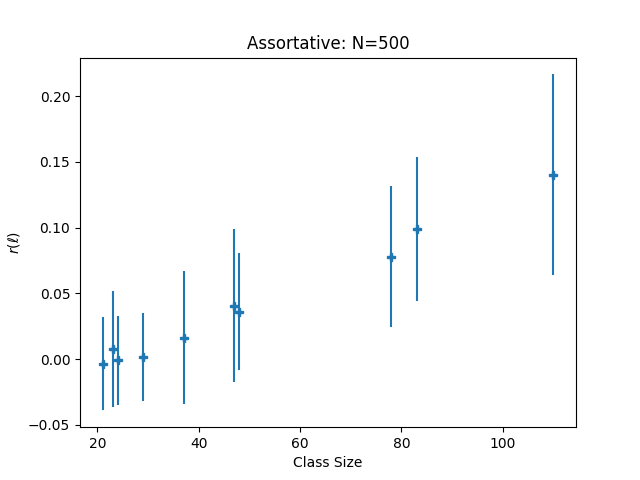
\includegraphics[width=0.5\textwidth]{assortative_N_500.png}
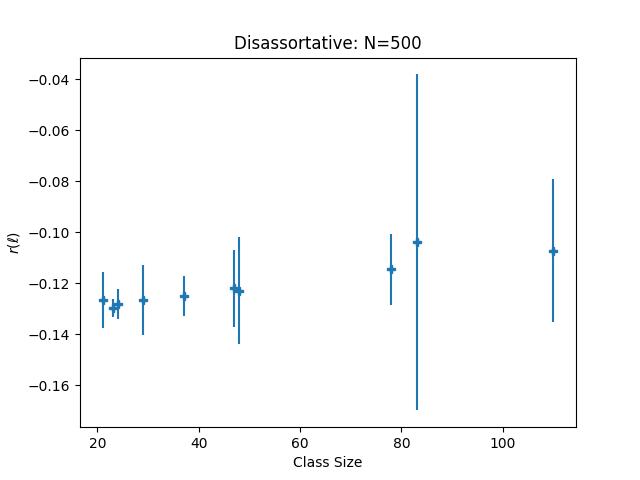
\includegraphics[width=0.5\textwidth]{disassortative_N_500.png}
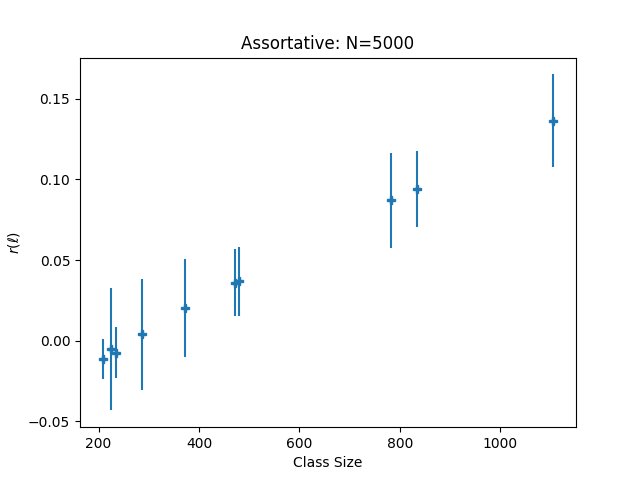
\includegraphics[width=0.5\textwidth]{assortative_N_5000.png}
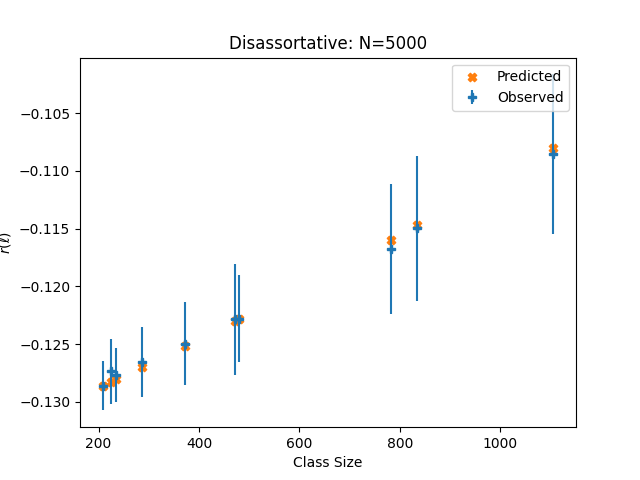
\includegraphics[width=0.5\textwidth]{disassortative_N_5000.png}
\caption{Distribution of $r(\ell)$ on DC-SBM random networks.  Errorbars show the standard deviation within each class}
\end{figure}

Figure NUMBER shows the distribution of $r_\ell$ within each class on a single DC-SBM for both assortatiive and disassortatiive nettworks.  Mean scores appear close to the theoretical prediction and the standard deviation decreases as the size of the network grows.  These networks were constructed in such a way that larger networks had higher mean degree, which decreases the impact of random fluctuations due to a small number of edges.  

\begin{figure}[h!]
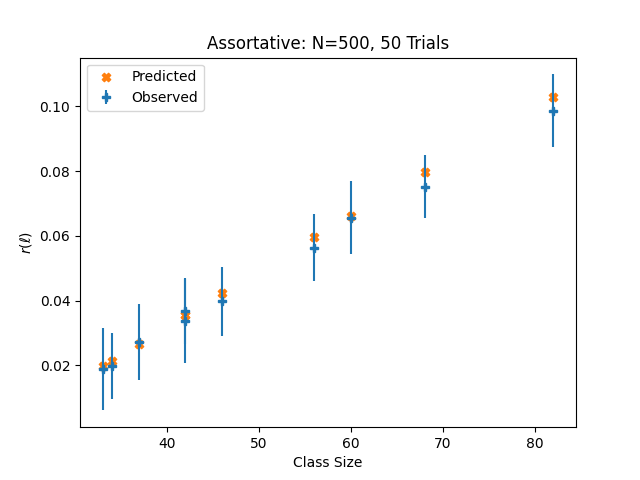
\includegraphics[width=0.5\textwidth]{assortative_N_500_trials_50.png}
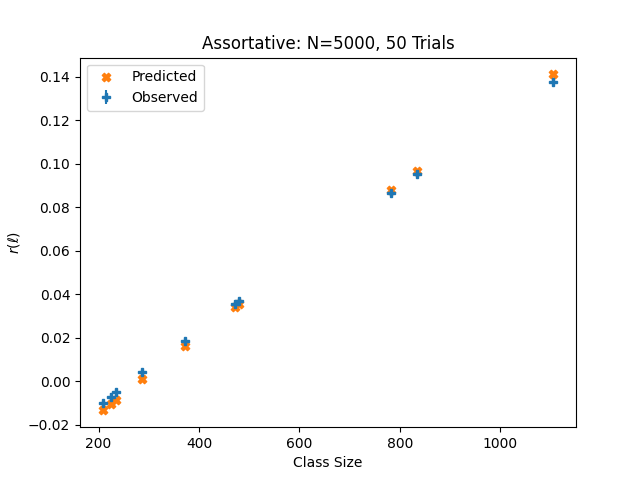
\includegraphics[width=0.5\textwidth]{assortative_N_5000_trials_50.png}
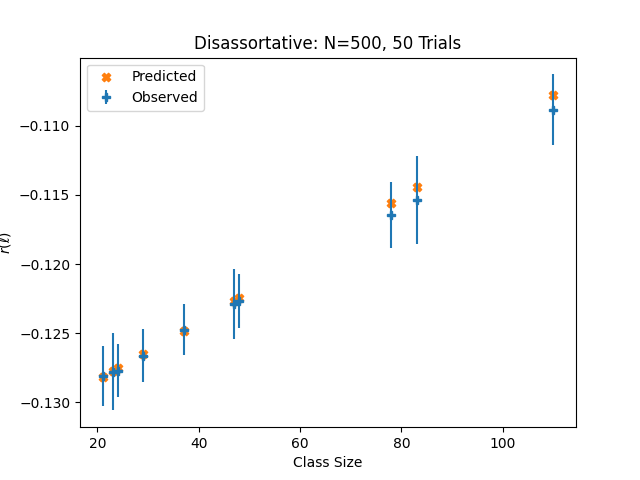
\includegraphics[width=0.5\textwidth]{disassortative_N_500_trials_50.png}
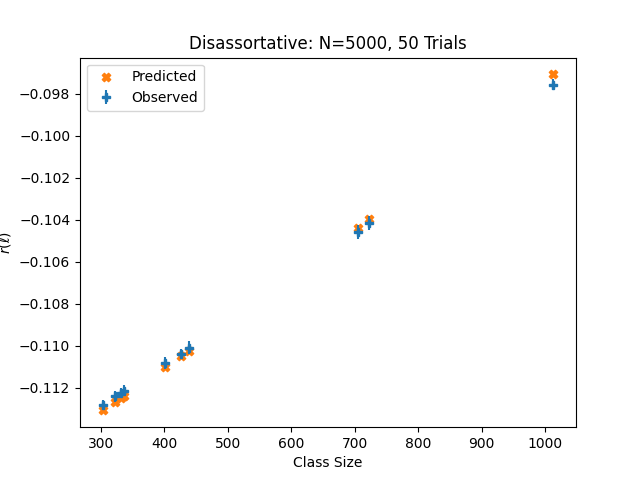
\includegraphics[width=0.5\textwidth]{disassortative_N_5000_trials_50.png}
\caption{Classwise mean $r(\ell)$ across 50 DC-SBM random networks}
\end{figure}

In figure NUMBER we consider the same unbalanced partition of classes, but compare the classwise mean of $r(\ell)$ scores across 50 different random networks generated from the same parameters.  Once again, $r(\ell)$ values appear to be centered around the theoretical prediction, and variance decreases as $n$ grows.  At $N=1000$ we begin to see the magnitude of the error in our theoretical analysis as the observed distribution converges.  It appears that the theoretical prediction slight underestimates $r(\ell)$ on small classes and overestimates it on large classes, for both assortative and disassortative and disassortative networks.

\begin{figure}[h!]
\includegraphics[width=0.5\textwidth]{assortative_N_500block_9.png}
\includegraphics[width=0.5\textwidth]{assortative_N_5000block_9.png}
\includegraphics[width=0.5\textwidth]{disassortative_N_500block_9.png}
\includegraphics[width=0.5\textwidth]{disassortative_N_5000block_9.png}
\caption{Distribution of $r(\ell)$ within one block of DC-SBM}
\end{figure}

In figure NUMBER we take a closer look at the distribution of $r_\ell$ within a single class of a single random network.  The distribution appears to be centered around the theoretical prediction.  It is unimodal, fairly symmetric and not very heavy-tailed, appearing similar in shape to a Poisson distribution.

\section{Discussion}

\bibliographystyle{plain} % We choose the "plain" reference style
\bibliography{refs} % Entries are in the refs.bib file

\section*{Code}

\end{document}